\documentclass[12pt,a4]{article}
\usepackage{physics, amsmath,amsfonts,amsthm,amssymb, mathtools,steinmetz, gensymb, siunitx}	% LOADS USEFUL MATH STUFF
\usepackage{xcolor,graphicx}
\usepackage[left=45pt, top=20pt, right=45pt, bottom=45pt ,a4paper]{geometry} 				% ADJUSTS PAGE
\usepackage{setspace}
\usepackage{caption}
\usepackage{tikz}
\usepackage{pgf,tikz,pgfplots,wrapfig}
\usepackage{mathrsfs}
\usepackage{fancyhdr}
\usepackage{float}
\usepackage{array}
\usepackage{booktabs,multirow}
\usepackage{bm}

\usetikzlibrary{decorations.text, calc}
\pgfplotsset{compat=1.7}

\usetikzlibrary{decorations.pathreplacing,decorations.markings}
\usepgfplotslibrary{fillbetween}

\newcommand{\vect}[1]{\boldsymbol{#1}}

\usepackage{hyperref}
%\usepackage[style= ACM-Reference-Format, maxbibnames=6, minnames=1,maxnames = 1]{biblatex}
%\addbibresource{references.bib}


\AtBeginDocument{\hypersetup{pdfborder={0 0 0}}}

\title{
\textsc{Topic 4}
}
\author{\textsc{J L Gouws}
}
\date{\today
\\[1cm]}



\usepackage{graphicx}
\usepackage{array}




\begin{document}
\thispagestyle{empty}

\maketitle

\begin{enumerate}
  \item
    \begin{enumerate}
      \item
        All the results are obtained with an RK4 integrator.
        Figure~\ref{fig:Lotka_Volterra} shows solutions to a Lotka-Volterra problem with different starting points.
        The particular problem is:
        \begin{align}
          \begin{split}
            \dot x &= 0.8 x + \alpha x^2 - xy\\
            \dot y &= - y + xy
          \end{split}
          \label{eq:lvprob}
        \end{align}
        \begin{figure}[H]
          \centering
          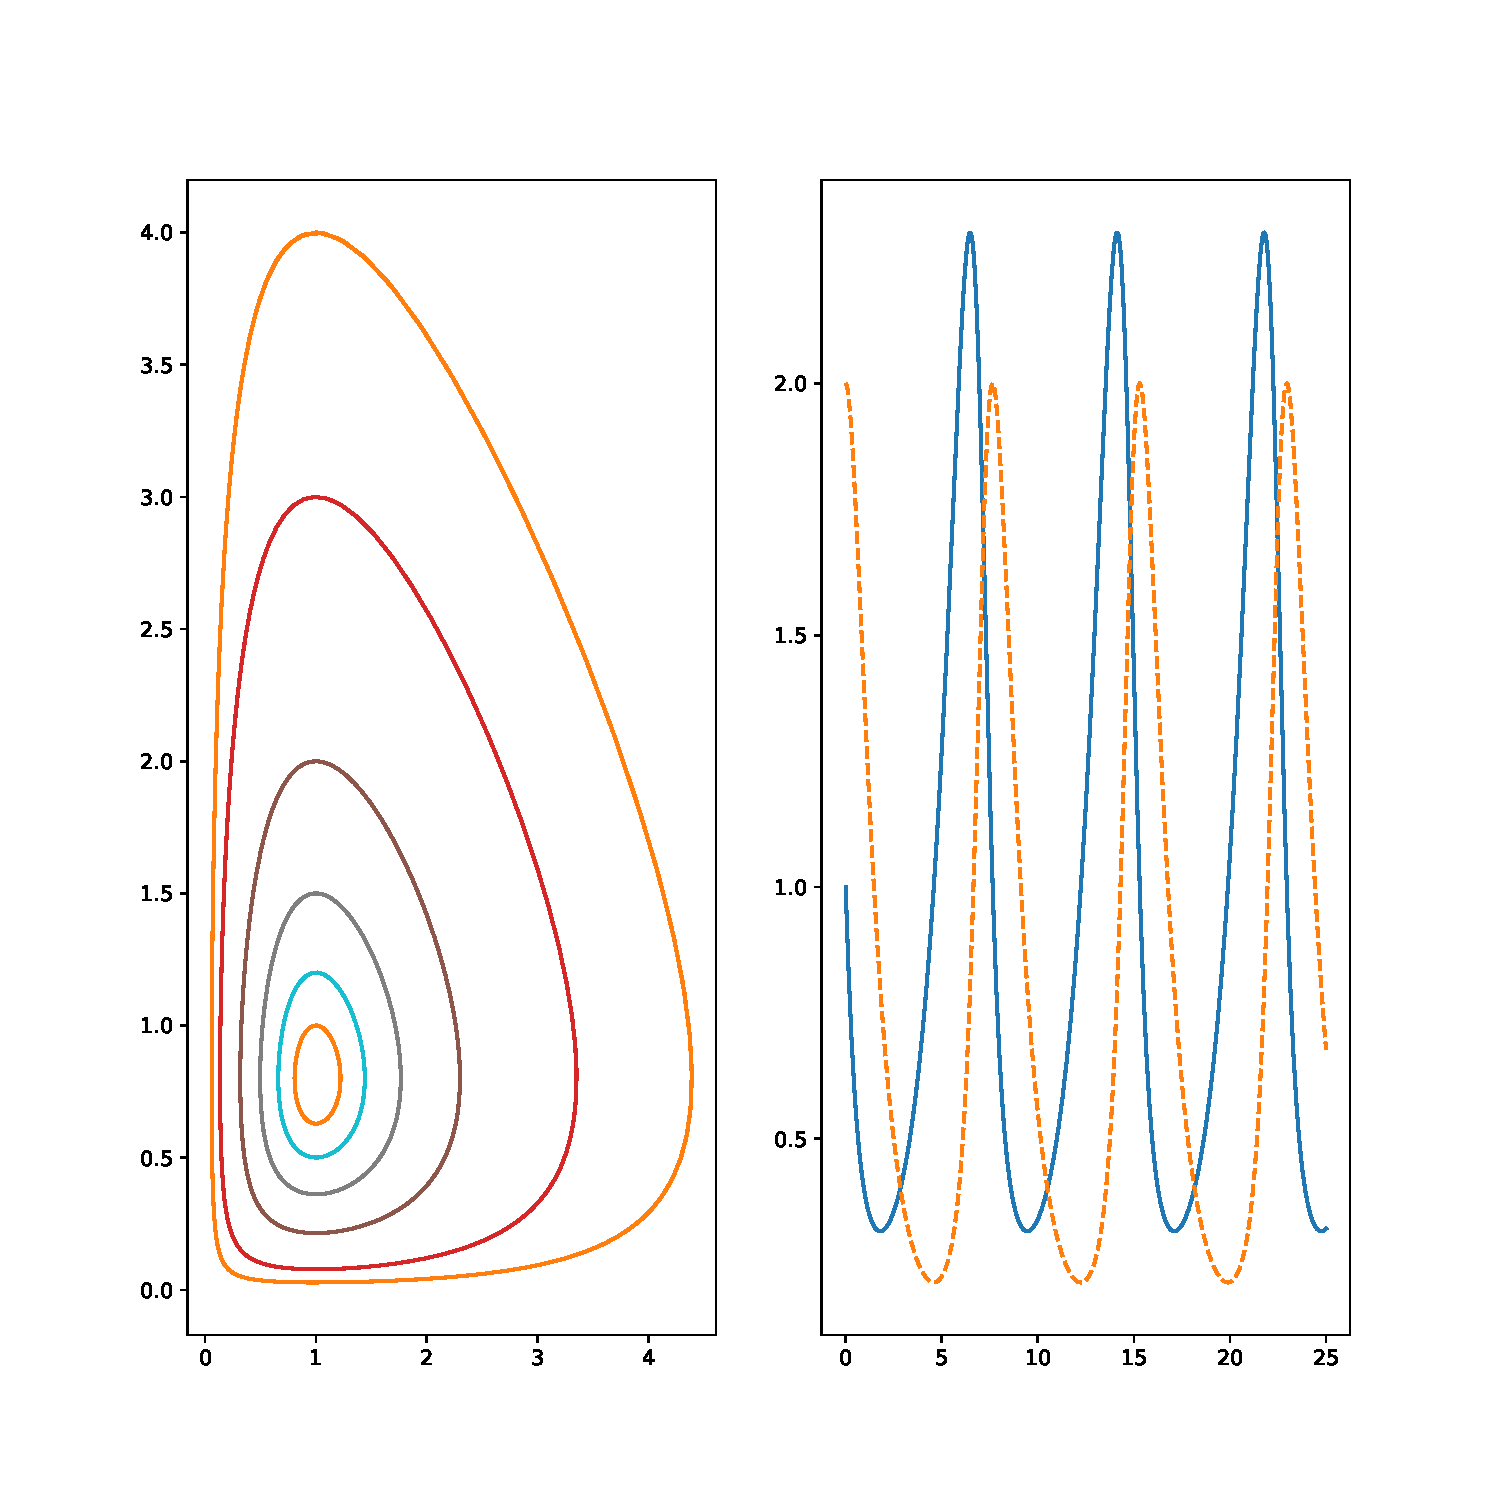
\includegraphics[scale = 0.6]{../figs/Lotka_Volterra.pdf} 
          \caption{Orbits of a Lotka Volterra system}
          \label{fig:Lotka_Volterra}
        \end{figure}

      \item
        Figure~\ref{fig:LVError} shows the value of $L$ for different initial values.
        \begin{equation*}
          L = f x + d \ln x - cy - a \ln y
        \end{equation*}

        \begin{figure}[H]
          \centering
          \includegraphics[scale = 0.6]{../figs/LVError.pdf}
          \caption{The value of $L$ along solutions}
          \label{fig:LVError}
        \end{figure}

      \item
        Figure~\ref{fig:Lotka_Volterra0.1} shows a numerical soution to a slightly perturbed problem, non-Hamiltonian problem.
        The problem sets $\alpha = 2 $ in Eq.~\ref{eq:lvprob}.
        \begin{figure}[H]
          \centering
          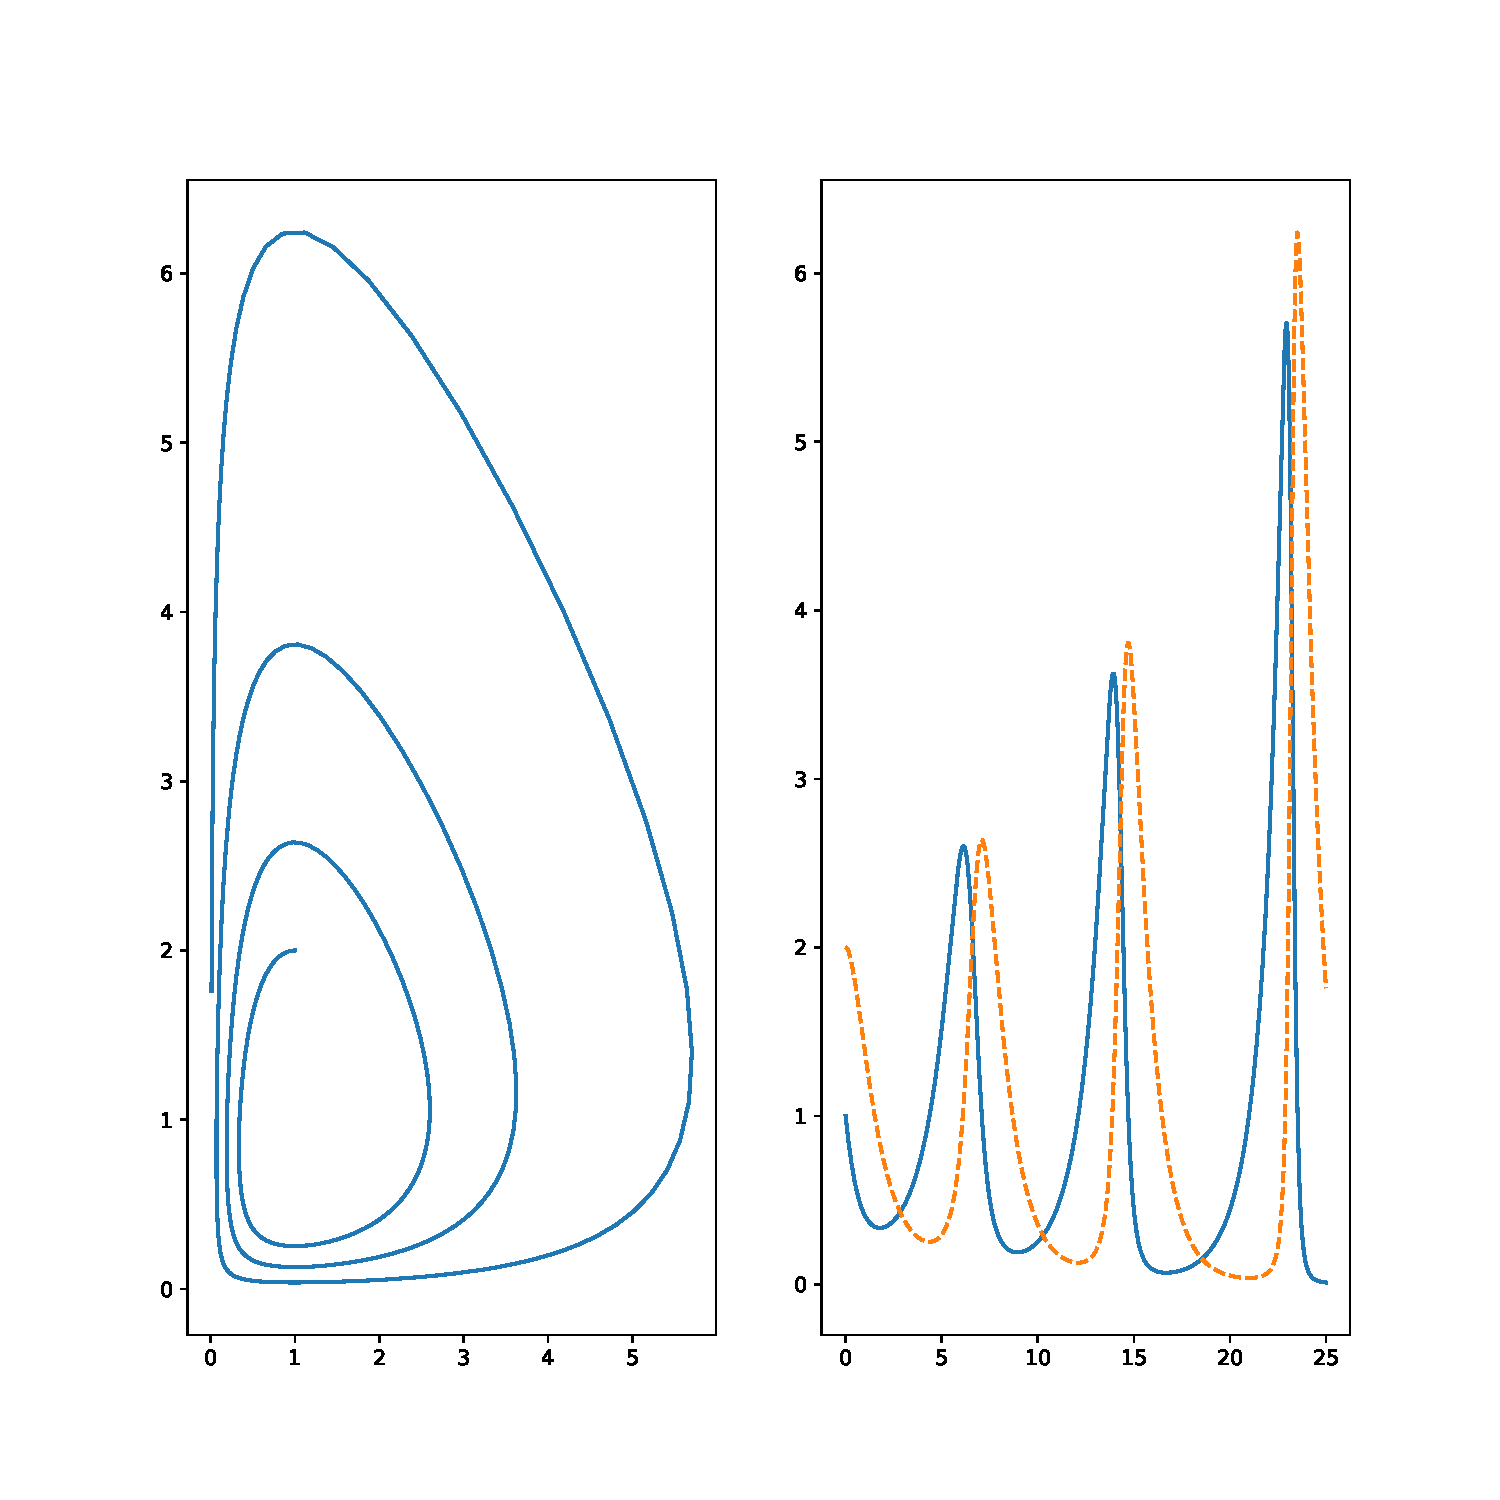
\includegraphics[scale = 0.6]{../figs/Lotka_Volterra0.1.pdf}
          \caption{Solution to the perturbed Lotka Volterra problem}
          \label{fig:Lotka_Volterra0.1}
        \end{figure}

    \end{enumerate}
  \item
    \begin{enumerate}
      \item
        Figure~\ref{fig:SIR} shows an SIR model's evolution through time.
        The particular problem is given by:
        \begin{gather*}
          \begin{split}
            \dot S &= - \beta S I + \sigma R\\
            \dot I &= \beta SI - \gamma I\\
            \dot R &= \gamma I - \sigma R
          \end{split}\\
          S(0) = \frac{8 \times 10 ^ 6 - 1}{8 \times 10^6},\qquad I(0) = \frac{1}{8 \times 10^6}, \qquad R(0) = 0
        \end{gather*}
        where $\beta =  0.8$ and $\gamma = 1 / 3$.
        \begin{figure}[H]
          \centering
          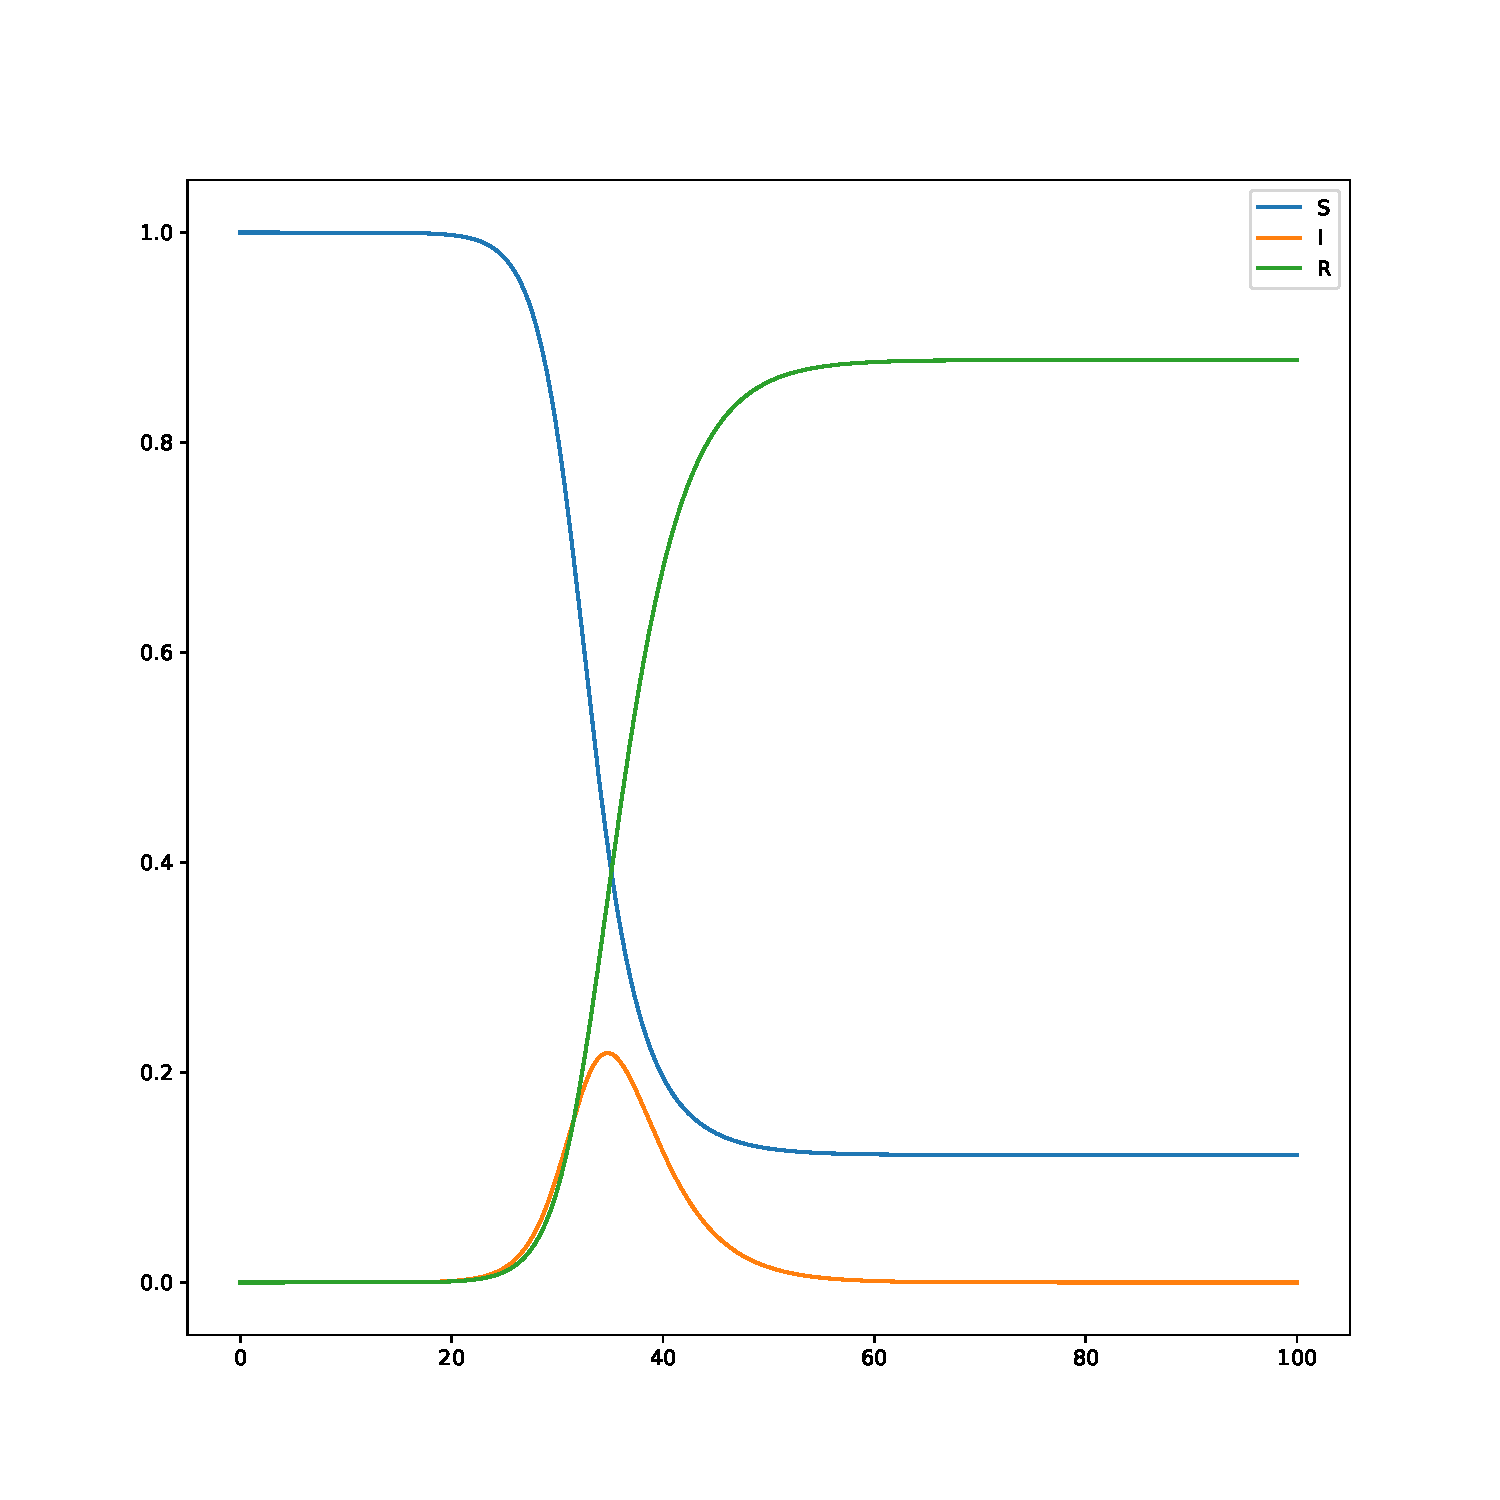
\includegraphics[scale = 0.8]{../figs/SIR.pdf}
          \caption{Evolution of an SIR model through time}
          \label{fig:SIR}
        \end{figure}
        \begin{enumerate}
          \item If the disease has these parameters, the infections peak after $t =  34.7500$ days.
          \item At the peak $\max\limits_{t}{I(t)} = 1748437$ people will be infected at the same time.
          \item After approximately $t =  99.5$ days, no single person should be infected.
          \item The proportion of people who will be infected is $p =  0.9$.
        \end{enumerate}

      \item
        Figure~\ref{fig:SIRbetaHalved} shows that halving $\beta$ (the contagiousness parameter) has a large impact on the infection curve.
        The curve is flatter and hence fewer people are infected at one time.
        This situation allows hospitals to keep up with new infections.
        \begin{figure}[H]
          \centering
          \includegraphics[scale = 0.8]{../figs/SIRbetaHalved.pdf}
          \caption{Evolution of an SIR model through time}
          \label{fig:SIRbetaHalved}
        \end{figure}
        \begin{enumerate}
          \item If the disease has these parameters, the infecaions peak at approximately $t =  197.2500$.
          \item At the peak $\max\limits_{t}{I(t)} = 117857$ people will be infected at the same time.
          \item After approximately $t =  417.9$ days, no single person should be infected.
          \item The proportion of people who will be infected is $p =  0.3$.
        \end{enumerate}
  \end{enumerate}
  \item
    \begin{enumerate}
      \item
        Lorenz models are sensitive to initial conditions.
        Figure~\ref{fig:xvtLorenz} illustrates the chaos exihibited by a Lorenz model.
        The lorenz model shown is:
        \begin{gather*}
          \begin{split}
            \dot x &= \sigma(y - x)\\
            \dot y &= rx - y - xz\\
            \dot z &= xy - bz
          \end{split}\\
          \sigma = 10 \qquad b = \frac{8}{3} \qquad r = 28
        \end{gather*}
        \begin{figure}[H]
          \centering
          \includegraphics[scale = 0.8]{../figs/xvtLorenz.pdf}
          \caption{Sensitivity of Lorenz system to initial conditions}
          \label{fig:xvtLorenz}
        \end{figure}
      \item
        Figure~\ref{fig:LorenzChaosTimeStep} illustrates the sensitivity solving of Lorenz model.
        The solution to the same Lorenz equations are substantially different solutions depending on the numerical integrator's time step.
        The errors and the actual solution are the same order.
        \begin{figure}[H]
          \centering
          \includegraphics[scale = 0.5]{../figs/LorenzChaosTimeStep.pdf}
          \caption{Chaos of Lorenz system when for different systems}
          \label{fig:LorenzChaosTimeStep}
        \end{figure}
      \item
        Figure~\ref{fig:lorenz} shows the Lorenz model settling into two lobes.
        \begin{figure}[H]
          \centering
          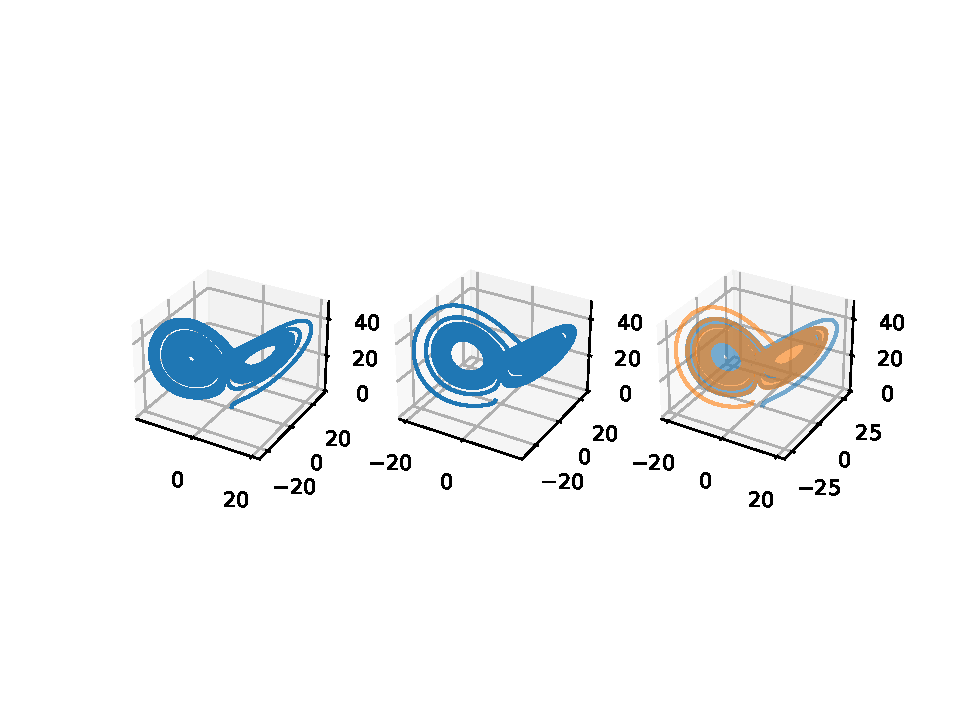
\includegraphics[scale = 0.7]{../figs/lorenz.pdf}
          \caption{3D plots of a Lorenz model}
          \label{fig:lorenz}
        \end{figure}
  \end{enumerate}
\end{enumerate}

\end{document}
